\documentclass[12pt]{article}
\usepackage{geometry}
\geometry{head=10mm,foot=10mm,left=20mm,right=20mm}

\usepackage{amsmath,amsthm,amssymb,scrextend}

\usepackage{fancyhdr}
\setlength{\headheight}{14.5pt}
\addtolength{\topmargin}{-2.5pt}
\pagestyle{fancy}

\usepackage{listings}
\usepackage{color}
\usepackage{xcolor}
\definecolor{codegreen}{rgb}{0,0.6,0}
\definecolor{codegray}{rgb}{0.5,0.5,0.5}
\definecolor{codepurple}{rgb}{0.58,0,0.82}
\lstset{
			backgroundcolor=\color{red!50!green!50!blue!50!white!20},
			breaklines = true,
			tabsize=2,
			commentstyle=\color{codegreen},
			keywordstyle=\color{magenta},
			numberstyle=\tiny\color{codegray},
			stringstyle=\color{codepurple},
	    }

\usepackage{graphicx}
\usepackage{float}
\usepackage{multicol}
\usepackage[colorlinks=true, pdfstartview=FitV, linkcolor=blue,
citecolor=blue, urlcolor=blue]{hyperref}

\begin{document}

\chead{Statistic Cheat Sheet}

    \section*{CH3. Single Variable Distribution}
        \subsection*{Probability mass function (pmf)}
        Given the range of \emph{discrete} random variable X $supp(X)\in R$, function $f(x): R\rightarrow [0,1]$ is defined as
        \begin{equation}
            f(x)=
            \begin{cases}
                P(X=x), \quad\ x \in supp(X)\\
                0, \quad\ \quad\ \quad\ \ \ \ x\notin supp(X)
            \end{cases}
        \end{equation}
        $f(x)$ satisfy:
        \begin{enumerate}
            \item $f(x)>0, \forall x \in supp(X)$
            \item $\sum_{x\in supp(X)}f(x)=1$
            \item $P(X\in A)=\sum_{x \in A}f(x)$, A$\in supp(X)$
        \end{enumerate} 
        And we can say that $f(x)$ is the pmf of X.
        \subsection*{Cumulative distribution function (CDF)}
        \begin{equation}
            F(x)=P(X\leq x)=\sum_{x_i\leq x}f(x)
        \end{equation}
        We can said that $F(x)$ is CDF.
        \newline
        CDF is `Cumulative' distribution function, so it's a nondecreasing function.
        \newline
        \newline
        Properties of discrete random variables' CDF
        \begin{enumerate}
            \item $P(X>a) = 1-P(X\leq a)= 1-F(a)$
            \item $P(X\geq a)= P(X=a)+P(X>a)=f(a)+1-F(a)=1-F(a)+f(a)$
            \item $P(a<X\leq b) = F(b)-F(a)$
            \item $P(a<X<b)=F(b)-f(b)-F(a)$
            \item $P(a\leq X \leq b)=F(b)-F(a)+f(a)$
            \item $P(a \leq X < b)=F(b)-F(a)+f(a)-f(b)$
            \item $\lim_{x \to -\infty}F(x)=0,\ \lim_{x\to\infty} F(x)=1$
        \end{enumerate}
        \subsection*{Probability density function}
        \begin{equation}
            P(a<x<b)=\int_{a}^b f(x)dx = [F(x)]_a^b =F(b)-F(a)
        \end{equation}
        $f(x)$ must satisfy
        \begin{enumerate}
            \item $f(x) > 0, \forall x \in supp(X)$
            \item $\int_{x \in supp(X)}f(x)dx = 1$
        \end{enumerate}
        Something important:
        \begin{itemize}
            \item You need to write down the range of x to get full score
            \item Point probability = 0
            \item $f(x)$ is height, not probability, so it may > 1
        \end{itemize}
        Because
        \begin{equation}
            \int_{a}^b f(x)dx  = [F(x)]_a^b
        \end{equation}
        We can see that
        \begin{equation}
            f(x)=\frac{\partial F(x)}{\partial x},\quad\ F(x)=\int_{-\infty}^xf(u)du
        \end{equation}
        \subsection*{Moments of random variables}
        Expected Value
        \begin{equation}
            E(x)=\int_{a}^bxf(x)dx
        \end{equation}
        Variance
        \begin{equation}
            \begin{aligned}
                Var(x)&=E\{[x-E(x)]^2\}=E\{x^2-2xE(x)-[E(x)]^2\}\\
                      &=E(x^2)-2[E(x)]^2+[E(x)]^2 = E(x^2)-[E(x)]^2
            \end{aligned}
        \end{equation}
        Quantile
        \newline
        \newline
        Given $0<p<1$, and $F(\cdot)$ is strictly increasing function, if
        \begin{equation}
            \pi_p=F^{-1}(p)
        \end{equation}
        $F(\pi_p) = P(X\leq \pi_p)=p$, then we can say $\pi_p$ is the $p-th$ quantile of r.v. X
        \newpage
        \hspace*{-6.2mm}Moment, central moment and standard moment
        \newline
        \newline
        Given $E(X)=\mu$, $Var(X)=\sigma^2$
        \begin{enumerate}
            \item $k-th$ moment: $E(X^k)$
            \item $k-th$ central moment: $\mu_k=E\big[(X-\mu)^k\big]$
            \item $k-th$ standard moment: $\gamma_k=E(Z_X^k)=E\bigg[(\frac{X-\mu}{\sigma})^k\bigg]=\frac{E[(X-\mu)^k]}{\sigma^k}$
        \end{enumerate}
        \subsection*{Moment generating function}
        \begin{equation}
            M_X(t)=E(e^{tX})=
            \begin{cases}
                \sum_{x}e^{tx}f(x)=\sum_xe^{tx}P(X=x)\\
                \int_xe^{tx}f(x)dx
            \end{cases}
        \end{equation}
        To calculate moment by MGF
        \begin{equation}
            E(X^k)=M_X^{(k)}(t)|_{t=0}
        \end{equation}
        Linear combination of MGF
        \newline
        Let $Y=aX+b$
        \begin{equation}
            M_Y(t)=E(e^{tY})=E[e^{t(aX+b)}]=E[e^{tb}e^{atX}]=e^{bt}M_X(at)
        \end{equation}
        Cumulant generating function
        \newline
        Let $K_X(t)=\ln M_X(t)$
        \begin{enumerate}
            \item $K'_X(t)|_{t=0}=E(X)$
            \item $K''_X(t)|_{t=0}=Var(X)$
            \item $K'''_X(t)|_{t=0}=E([X-E(X)]^3)$
            \item $K''''_X(t)|_{t=0}=E([X-E(X)^4])-3[Var(X)]^2$
        \end{enumerate}
        \subsection*{Jacobian transformation method}
        Step1. Inverse function: get $x=g^{-1}(y)$, and check if it's 1 to 1.
        \newline
        Step2. Jacobian: calculate $|J|=|\frac{\partial g^{-1}(y)}{\partial y}|$
        \newline
        Step3. Range: from $supp(X)$ and $g(y)$ get the range of new variable
        \newline
        Step4. Substitute: get $f_Y(y)=f_X[g^{-1}(y)]\times |J|$
        \subsection*{Truncated distribution}
        \begin{equation}
            f(x|X\leq a)=\frac{f(x)}{F(a)},\ x\leq a
        \end{equation}
        \begin{equation}
            f(x|X\geq a)=\frac{f(x)}{1-F(a)},\ x\geq a
        \end{equation}
        \begin{equation}
            f(x|a \leq X \leq b)=\frac{f(x)}{F(b)-F(a)},\ a \leq X \leq b
        \end{equation}
        \subsection*{Jensen's inequality}
        if $g(\cdot)$ satisfy $g[(1-\alpha)x+\alpha y] > (1-\alpha)g(x)+\alpha g(y)$, it's a strictly concave function. Then
        \begin{equation}
            E[g(X)] < g[E(X)]
        \end{equation}
        if $g(\cdot)$ satisfy $g[(1-\alpha)x+\alpha y] < (1-\alpha)g(x)+\alpha g(y)$, it's a strictly conves function. Then
        \begin{equation}
            E[g(X)] > g[E(X)]
        \end{equation}
        if $g(\cdot)$ satisfy $g[(1-\alpha)x+\alpha y] = (1-\alpha)g(x)+\alpha g(y)$, it's a linear function. Then
        \begin{equation}
            E[g(X)] = g[E(X)]
        \end{equation}
        \begin{figure}[H]
            \centering
            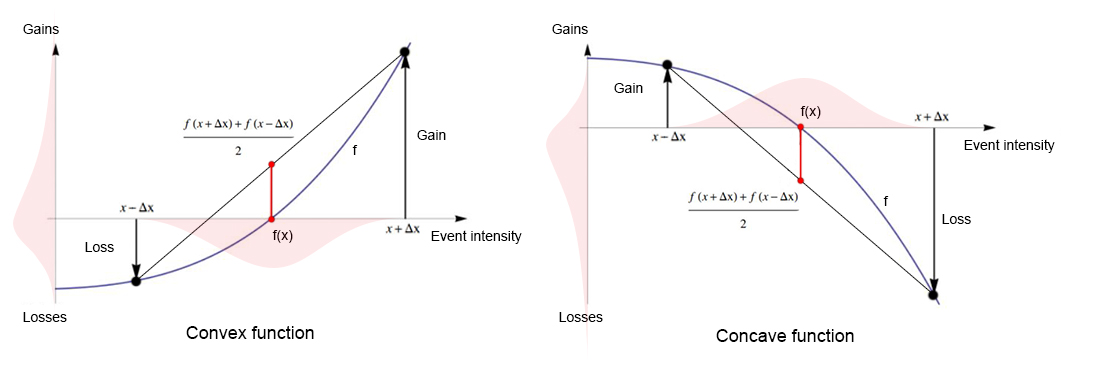
\includegraphics[width = \textwidth]{jensen_eng.jpeg}
            \caption{Jensen's Inequality}
        \end{figure}
\end{document}
